\documentclass{article}
\usepackage{a4wide}
\usepackage{amsmath}
\usepackage{url}
\usepackage{amssymb}
\usepackage{clrscode3e}
\usepackage{tikz}
\usepackage{bm}
\usepackage{graphicx}
\graphicspath{ {./images/} }

\title{Homework 6}
\author{Joni Vrapi}
\date{11/26/2022}

\begin{document}

\maketitle

\textbf{Statement of Integrity:} I, Joni Vrapi, attempted to answer each question honestly and to the best of my abilities. I cited any, and all, help that I received in completing this assignment.

\hfill

\textbf{Problem 1.} A tree, by definition \cite{website:1}, is a type of graph in which any two vertices are connected by exactly one path and in which there are no cycles. In other words, a connected acyclic graph. We know that the edges in $E$ are undirected. We also know that both bfs and dfs produce the same tree $T$ which we will assume $G \neq T$. 

If we therefore assume that $G$ is connected but not a tree, then it must contain a cycle $C$. If $C$ has $n$ nodes $u_1, u_2, ... , u_n$, then $C$ represents the cycle $u_1 \rightarrow u_2 \rightarrow ... \rightarrow u_n \rightarrow u_1$. If we assume that bfs and dfs encounter the cycle at node $u_i$, then dfs will add edges $(u_1, u_2), ... , (u_{i-2}, u_{i-1})$ while bfs will start by adding edges $(u_1, u_2), (u_1, (u_i))$. Since we can see that this contradicts the assumption that bfs and dfs have equal trees, we can see that bfs and dfs have equal trees iff the input graph is also a tree. Therefore, $G = T$.

\hfill

\textbf{Problem 2a.} If we have a bipartite graph $G$ where $p_n$ signifies a person, and $d_n$ signifies a cooking day, then a directed edge $(p_i, d_j)$ between them signifies if person $p_i$ is able to cook on day $d_j$. 

\begin{center}
    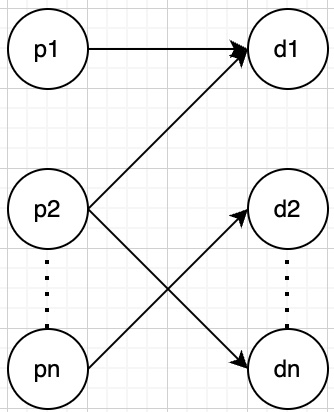
\includegraphics[width=4cm, height=5cm]{images/bipartite-graph.jpg}
\end{center}

In order to find out whether this bipartite graph has a perfect matching, we can use the Maximum Flow Algorithm \cite{website:2}. In order to set this up, we must add 2 more nodes (a source node $s$, and a sink node $t$) to our bipartite graph like so:

\begin{center}
    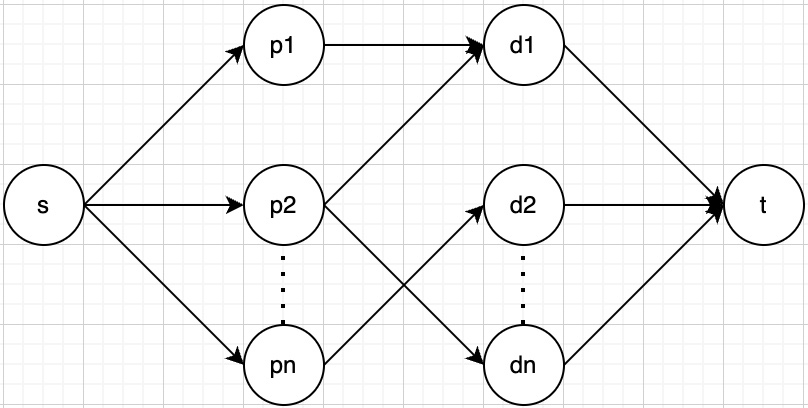
\includegraphics[width=10cm, height=5cm]{images/maximum-flow-graph.jpg}
\end{center}

If we set each edge's weight to be $1$, then the schedule will be feasible iff the maximum flow is $n$ and the number of edges in $G$ is also $n$.

\hfill

\textbf{Problem 2b.} First, we would construct the bipartite graph $G$ from (a). It takes $O(1)$ time to decide if $(p_i, d_j))$ should be an edge so the total time to build the graph would be $O(n^2)$. If we let $R$ denote the set of edges given to us by Renee, we can delete the edge $(p_j, d_k)$ to obtain $R'$ which would have a size of $n-1$ and have no person or day appear more than once. From \cite{website:3} we need to find an augmenting path with respect to $R'$ in $O(|E|) = O(n^2)$ time. If we find an augmenting path, then this gives us a perfect matching and would correspond to a feasible dinner. If we do not find an augmenting path, then it would hold that $R'$ is a maximum matching in $G$ and there would be no perfect matching -- and therefore no feasible dinner schedule. 

\hfill

\textbf{Problem 3.} The algorithm \cite{website:3} begins by scanning through the ordered triples, maintaining an array pointing to linked lists which are associated to each computer $C_a$. For each triple, we create two nodes $(C_i, t_k), (C_j, t_k)$ and directed edges between them in both directions. We also append (to their respective list) each $C$ node. If it is not the first triple for $C_x$, then we include an edge from $(C_x, t)$ to $(C_x, t_k)$ where $t$ is the timestamp of the previous element. By doing this, we are able to construct these new nodes in constant time per ordered triple.

Now, if we want to decide if computer $C_a$ at time $x$ could have infected $C_b$ by time $y$, we would walk through the list we created above for $C_a$ until we reach the last node, and then run a directed BFS from that node to determine all nodes that are reachable from it. If the node $(C_b, y'); y' \leq y$ is reachable, we can say that it was infected, otherwise we would say that it has not been infected.

In terms of time complexity, each triple that is parsed results in a constant number of nodes and edges added to the graph, so the graph has $O(m)$ nodes and edges. It takes a constant amount of time to build it per node and edge -- also $O(m)$. Finally, running BFS takes a linear amount of time in the size of the graph which is also $O(m)$.

Finally, is the algorithm correct? The algorithm claims that if there are a sequence of paths between $C_a$ and $C_b$ then $C_b$ could have been infected by time $y$. Due to the way we are maintaining the lists of paths on a per-computer basis, and the fact that each time the virus moves from one computer to another, we are adding an edge between that computer and the next, there will always be a sequence of paths which describe the movements of the virus based on the given ordered triples. Knowing that there will always be $y'' \leq y \leq y'$ time for which the virus arrives at the next computer, it is obvious that we can build a sequence of edges that would result in a complete path. 

\hfill

\textbf{Problem 4a.} This problem can be modeled as a maximum flow network problem, much like problem 1. If we constructed a flow network with edges of weight 1 from the source, through $X$ and all the way into $S$, then the edges from $S$ into the sink would be of weight $|X|$. From source to $X$, as well as from $S$ to sink, there should be $|X|$ edges. From here we can use Ford-Fulkerson \cite{website:4} to compute the maximal flow in $O(V*E^2)$ time. If the maximal flow is equal to $|X|$, then there exists an evacuation route.

\hfill

\textbf{Problem 4b.} We could solve for this extra condition by splitting up each vertex $v$ in $G$ into a set of 2 vertices $v_i$ and $v_j$. All in-edges of $v$ will point to $v_i$ while all out-edges of $v$ will leave from $v_j$, and a single out-edge will leave from $v_i$ and point to $v_j$. We will weight these edges the same as in problem (4a) and re-run Ford-Fulkerson, with the condition that no two paths can share an edge now meaning that no two paths can share the internal edge between $v_i$ and $v_j$. We can then shrink the $(v_i, v_j)$ pairs back to produce a set of node-disjoint paths. The most simple example where the answer is "yes" to (a) and "no" to (b) is the following:

\begin{center}
    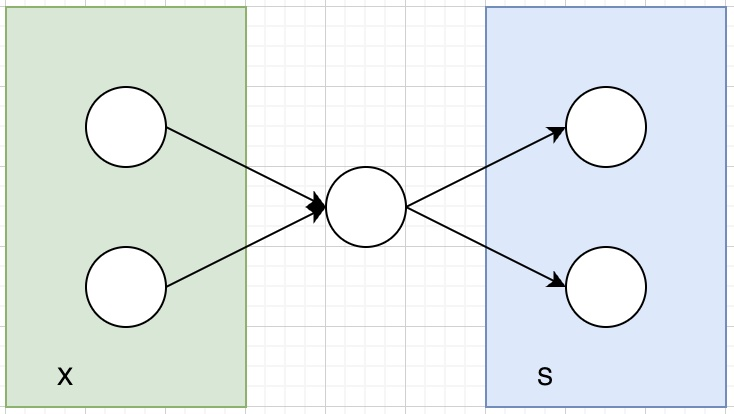
\includegraphics[width=9cm, height=5cm]{images/problem-4-example.jpg}
\end{center}

\newpage
\bibliography{citation} 
\bibliographystyle{ieeetr}

\end{document} 
